\clearpage
\subsubsection{Goto} % (fold)
\label{sub:goto}

The last jump statement is the goto statement. This is an unstructured jump, allowing you to jump anywhere in the code. Structured Programming principles called for the abolition of the goto statement. This is a statement you need to be aware of, but not one that should be used.

\begin{figure}[h]
   \centering
   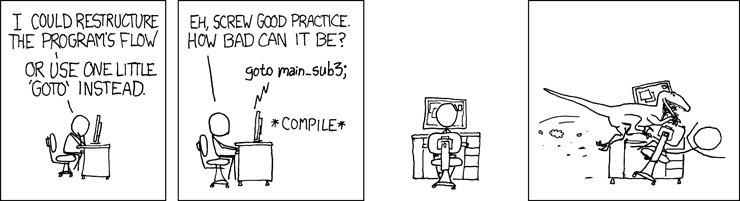
\includegraphics[width=\textwidth]{./topics/control-flow/images/goto} 
   \caption{The dangers of using goto, from \url{http://xkcd.com/292/}}
   \label{fig:goto}
\end{figure}

\mynote{
\begin{itemize}
  \item Goto is an action that allows you to jump to another instruction and continue from there.
  \item You need to be aware of the goto statement, but you should not use it.
\end{itemize}
}

% subsection goto (end)